\documentclass[hidelinks,11pt,dvipsnames]{article}
% xcolor commonly causes option clashes, this fixes that
\PassOptionsToPackage{dvipsnames,table}{xcolor}
\usepackage[tmargin=1in, bmargin=1in, lmargin=0.8in, rmargin=1in]{geometry}

%%%%%%%%%%%%%%%%%%%%%%%%%%%%%%%%%%%%%%%%%%%%%%%%%%%%%%%%%%%%%%%%%%%%
%%% For inkscape-figures
%%% Assumes the following directory structure:
%%% master.tex
%%% figures/
%%%     figure1.pdf_tex
%%%     figure1.svg
%%%     figure1.pdf
%%%%%%%%%%%%%%%%%%%%%%%%%%%%%%%%%%%%%%%%%%%%%%%%%%%%%%%%%%%%%%%%%%%%
%\usepackage{import}
\usepackage{pdfpages}
\usepackage{transparent}

\newcommand{\incfig}[2][1]{%
    \def\svgwidth{#1\columnwidth}
    \import{./figures/}{#2.pdf_tex}
}

\pdfsuppresswarningpagegroup=1

% enable synctex for inverse search, whatever synctex is
\synctex=1
\usepackage{float,macrosabound,homework,theorem-env}
\usepackage{microtype}


% font stuff
\usepackage{sectsty}
\allsectionsfont{\sffamily}
\linespread{1.1}

% bibtex stuff
\usepackage[backend=biber,style=alphabetic,sorting=anyt]{biblatex}
\addbibresource{main.bib}

% colored text shortcuts
\newcommand{\blue}[1]{\color{MidnightBlue}{#1}}
\newcommand{\red}[1]{\textcolor{Mahogany}{#1}}
\newcommand{\green}[1]{\textcolor{ForestGreen}{#1}}


% use mathptmx pkg while using default mathcal font
\DeclareMathAlphabet{\mathcal}{OMS}{cmsy}{m}{n}

% fixes the positioning of subscripts in $$ $$
\renewcommand{\det}{\operatorname{det}}

\usetikzlibrary{positioning, arrows.meta}
\newcommand{\here}[2]{\tikz[remember picture]{\node[inner sep=0](#2){#1}}}

%%%%%%%%%%%%%%%%%%%%%%%%%%%%%%%%%%%%%%%%%%%%%%%%%%%%%%%%%%%%%%%%%%%%%
%%% Entry Counter
%%%%%%%%%%%%%%%%%%%%%%%%%%%%%%%%%%%%%%%%%%%%%%%%%%%%%%%%%%%%%%%%%%%%%
\newcounter{entry-counter}
\newcommand{\entry}[1]
{
	\addtocounter{entry-counter}{1}
    \tchap{Entry \arabic{entry-counter}}
	%\addcontentsline{toc}{section}{Entry \arabic{entry-counter}: #1}
	\vspace{-1.5em}
    \begin{center}
		\small \emph{Written: #1}
    \end{center}
}

\usepackage{titling}
\renewcommand\maketitlehooka{\null\mbox{}\vfill}
\renewcommand\maketitlehookd{\vfill\null}

\usepackage{indentfirst}

% Title page stuff
\title{Ising in the Tropics}
\date{}
%\author{Author Name}
%\use package[show frame]{geometry}

\usepackage{titling}
\renewcommand\maketitlehooka{\null\mbox{}\vfill}
\renewcommand\maketitlehookd{\vfill\null}
\begin{document}
\setcounter{page}{1}
\setcounter{section}{-1}
\maketitle

\newpage

\tableofcontents
\newpage

\section{Introduction}
The reverse Ising problem is special case of a more general problem in mathematics: a ``horribly nasty optimization problem''. It is worth noting that ``horribly nasty'' here is a colloquial term for ``exponentially worsening,'' by which we mean the number of expressions we wish to optimize grows exponentially in the number of variables. Suffice to say that ``horribly nasty'' does not fully encapsulate the true horror of our predicament, but then again, scientists have never been known for their ability to name things.

One of the only approaches available to the poor sod facing a horribly nasty optimization problem is to try random stuff. As the saying goes, desperate times call for flinging anything and everything in all directions at once. Sticking to the wall isn't necessarily the goal, rather, one hopes to establish that there is indeed a wall upon which to stick. It is with this spirit that we return to the foundations of the reverse Ising problem itself and propose yet another technical formulation. Foundations offer stability, reassuring generality and an all around nice feeling. What else feels nice? That's right, the \emph{tropic}...al semiring. The analogy doesn't make any sense and once again you can blame the broader scientific community for their utter inability to name things. It's not my fault, they made me this way. 

Anyways, tropical geometry is a natural setting for optimization problems because inequalities are baked into its algebra. As the reader likely knows, in tropical geometry we replace the normal binary operations of addition and multiplication on the reals with minimization and addition. Why don't we replace multiplication with minimization and leave addition unchanged, you ask? If you didn't ask so many annoying questions then you'd likely have more friends, I answer (the actual answer is valuations, logarithms and limits, but I'm lazy and didn't want to justify that). I direct you to Figure \ref{fig:no-friends}. Besides the canned "tropical arithmetic = natural choice for optimization" justification, the actual motivation for this document is ``Isaac is taking a tropical geometry class and was excited to apply it to Ising.'' Providing compelling motivation for a piece of mathematics is yet another seemingly routine task at which mathematicians typically fail, and I once again deflect the blame upon those who taught me.
\begin{figure}[ht]
    \centering
	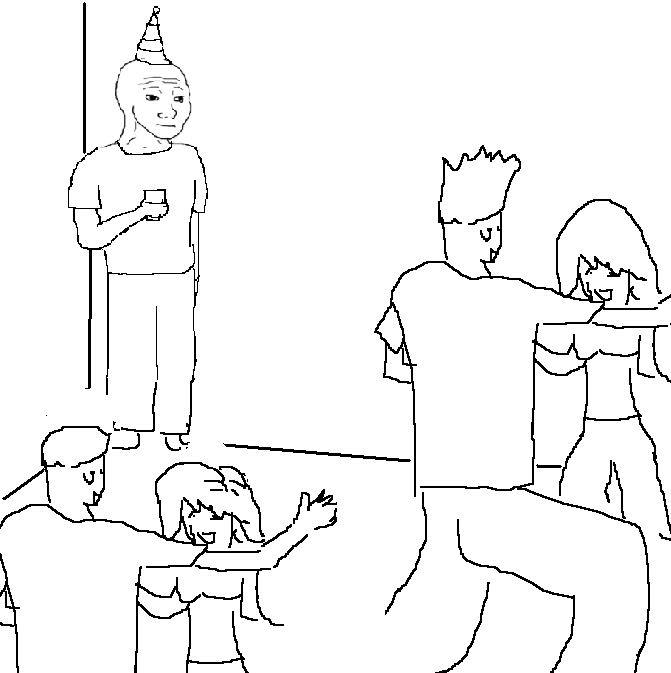
\includegraphics[width=6cm]{./figures/no-friends-at-party.png}
    \caption{``No one talks to me (the reader) because I ask annoying questions that are hard to answer.''}
	\label{fig:no-friends}
\end{figure}

With our feelings sufficiently hurt and our lack of solid justification adequately exposed, we proceed to writing down stuff that looks like math. We start with a brief review of tropical arithmetic before launching directly into a tropical formulation of reverse Ising. This adds absolutely nothing new, except perhaps a new angle and a new set of theorems to try and apply.

\section{Reformulating Ising in the Tropical Semiring}
\begin{defn}\label{defn:tropical-semiring}
	The \textbf{tropical semiring} $(\bR \cup \{\infty\},\oplus,\odot)$ is a \href{https://en.wikipedia.org/wiki/Semiring}{\underline{semiring}} (sometimes called a ``rig'' because it's a ring without \underline{n}egatives and because it's funnier) whose addition is ``$\min$'' and whose multiplication is regular addition on the reals. That is,
	\begin{align*}
		a \oplus b &:= \min\{a,b\} \\
		a\odot b &:= a + b.
	\end{align*}
	We note that for any $a \in \bR\cup \{\infty\}$, $a\oplus \infty = \infty$ and $a\odot 0 = a + 0 = a$, so $\infty$ is the additive identity and $0$ is the multiplicative identity. It then follows from that $a\odot \infty = \infty$.
\end{defn}
\begin{example}\label{example:some-tropical-operations}$ $
	\begin{itemize}
		\item $16 \oplus -5 = -5$
		\item $\frac{1}{2} \otimes (5 \oplus 4 \odot 6) = \frac{1}{2}(5 \oplus 10) = \frac{1}{2} \odot 5 = \frac{11}{2}$
		\item If $f(x) = x \oplus 2$, then $f(x) = x$ for $x < 2$ and $f(x) = 2$ for $x \geq 2$.
	\end{itemize}
\end{example}
The final item above is an example of a \emph{tropical polynomial}. We'll define these more generally in a second. First, we introduce some more notation: tropical exponents (over the integers) and tropical monomials.
\begin{defn}\label{defn:tropical-monomials}
	If $x \in \bR\cup \{\infty\}$ and $d \in \bZ$. If $d > 0$, then
	\begin{align*}
		x^{\odot d} = \overbrace{x\odot...\odot}^{\text{$d$-times}} = d\cdot x
	\end{align*}
	where $\cdot$ is the normal product on $\bR$. If $d< 0$, then $x^{\odot d} = (-x)^{\odot |d|} = d\cdot x$ and if $d = 0$ then $x^{\odot d} = 0$.

	A \textbf{tropical monomial} is a function $f:\bR^n\to \bR$ of the form 
	\begin{align*}
		f(x_1,...,x_n) = a\odot x_1^{\odot d_1}\odot...\odot x_n^{\odot d_n}
	\end{align*}
	for some $a \in \bR$ and $d_i \in \bZ$.	
\end{defn}
This is a lot of weird notation for something that we already understand quite well: tropical monomials are simply affine linear functions. Indeed, if we rewrite the definition above in terms of more familiar operations, we see that
\begin{align*}
	f(x_1,...,x_n) 
	&= a\odot x_1^{\odot d_1}\odot...\odot x_n^{\odot d_n} \\
	&= a\odot d_1x_1\odot ... \odot d_n x_n \\
	&= d_1x_1 + ... + d_nx_n + a.
\end{align*}
This looks a lot less scary, and is indeed something we readily understand. We can now define tropical polynomials.
\begin{defn}\label{defn:tropical-polynomial}
	A \textbf{tropical polynomial} is simply a polynomial over the tropical rig. Explicitly, it is a function $f:\bR^n \to \bR$ of the form
	\begin{align*}
		f(x_1,...,x_n) = (a_1\odot x_1^{\odot d_{11}}\odot...\odot x_n^{\odot d_{n1}} ) \oplus...\oplus (a_m\odot x_1^{\odot d_{1m}}\odot...\odot x_n^{\odot d_{nm}} ),
	\end{align*}
	i.e. it is a tropical sum of finitely many tropical monomials.
\end{defn}
\section{Appendix}

\printbibliography
\end{document}
